\documentclass[12pt,letterpaper]{hmcpset}
\usepackage[margin=1in]{geometry}
\usepackage{graphicx}
\usepackage{siunitx}

% info for header block in upper right hand corner
\name{ }
\class{Math 60}
\assignment{HW 11}
\duedate{Wednesday, June 1, 2016}

\newcommand{\f}[2]{\frac{#1}{#2}}
\newcommand{\bb}[1]{\mathbb{#1}}
\newcommand{\pn}[1]{\left(#1\right)}
\newcommand{\abs}[1]{\left|#1\right|}
\newcommand{\bk}[1]{\left[#1\right]}
\renewcommand{\bf}[1]{\mathbf{#1}}
\renewcommand{\labelenumi}{{(\alph{enumi})}}

\begin{document}

\problemlist{6.2.\{13, 15\}, 6.3.\{1, 3, 4, 25, 33\}}

\begin{problem}[Colley 6.2.13]
    Evaluate $\oint_C(x^4y^5-2y)~dx+(3x+x^5y^4)~dy$, where $C$ is the
    oriented curve pictured in Figure 6.29.
    \begin{center}
        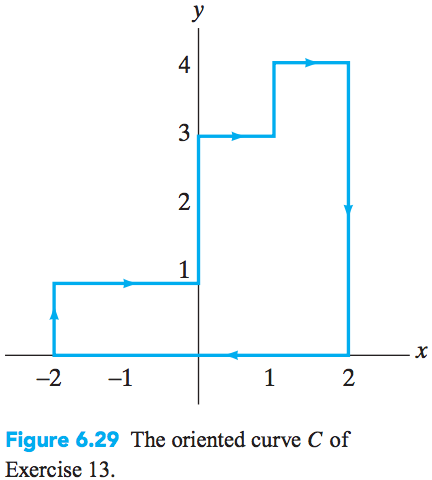
\includegraphics[scale=0.8]{img/6_2_13}
    \end{center}
\end{problem}
\begin{solution}
    \vfill
\end{solution}
\newpage

\begin{problem}[Colley 6.2.15]
    \begin{enumerate}
        \item Sketch the curve given parametrically by
            $\bf{x}(t)=(1-t^2,t^3-t)$.
        \item Find the area inside the closed loop of the curve.
    \end{enumerate}
\end{problem}
\begin{solution}
    \vfill
\end{solution}
\newpage

\begin{problem}[Colley 6.3.1]
    Consider the line integral $\int_Cz^2~dx+2y~dy+xz~dz$.
    \begin{enumerate}
        \item Evaluate this integral, where $C$ is the line segment
            from $(0,0,0)$ to $(1,1,1)$.
        \item Evaluate this integral, where $C$ is the path from
            $(0,0,0)$ to $(1,1,1)$ parametrized by
            $\bf{x}(t)=(t,t^2,t^3),~0\leq t\leq1$.
        \item Is the vector field
            $\bf{F}=z^2~\bf{i}+2y~\bf{j}+xz~\bf{k}$ conservative? Why
            or why not?
    \end{enumerate}
\end{problem}
\begin{solution}
    \vfill
\end{solution}
\newpage

\begin{problem}[Colley 6.3.3]
    In Exercises 3-17, determine whether the given vector field
    $\bf{F}$ is conservative. If it is, find a scalar potential
    function for $\bf{F}$.
    \[
        \bf{F}=e^{x+y}~\bf{i}+e^{xy}~\bf{j}
    \]
\end{problem}
\begin{solution}
    \vfill
\end{solution}
\newpage

\begin{problem}[Colley 6.3.4]
    In Exercises 3-17, determine whether the given vector field
    $\bf{F}$ is conservative. If it is, find a scalar potential
    function for $\bf{F}$.
    \[
        \bf{F}=2x\sin y~\bf{i}+x^2\cos y~\bf{j}
    \]
\end{problem}
\begin{solution}
    \vfill
\end{solution}
\newpage

\begin{problem}[Colley 6.3.25]
    Let $\bf{F}=x^2~\bf{i}+\cos y\sin z~\bf{j}+\sin y\cos z~\bf{k}$.
    \begin{enumerate}
        \item Show that $\bf{F}$ is conservative and find a scalar
            potential function $f$ for $\bf{F}$.
        \item Evaluate $\int_{\bf{x}}\bf{F}\cdot d\bf{s}$ along the
            path $\bf{x}:[0,1]\to
            \bb{R}^3,~\bf{x}(t)=(t^2+1,e^t,e^{2t})$.
    \end{enumerate}
\end{problem}
\begin{solution}
    \vfill
\end{solution}
\newpage

\begin{problem}[Colley 6.3.33]
    \begin{enumerate}
        \item Determine where the vector field
            \[
                \bf{F}=\f{x+xy^2}{y^2}~\bf{i}-\f{x^2+1}{y^3}~\bf{j}
            \]
            is conservative.
        \item Determine a scalar potential for $\bf{F}$.
        \item \begin{sloppypar} Find the work done by $\bf{F}$ in
            moving a particle along the parabolic curve ${y=1 +x-x^2}$
            from $(0,1)$ to $(1,1)$.\end{sloppypar}
    \end{enumerate}
\end{problem}
\begin{solution}
    \vfill
\end{solution}
\end{document}
